% ============================================================
%  Chapter 4 — Methodology
% ============================================================
\chapter{Methodology}
\label{ch:methodology}

%-------------------------------------------------------------
\section{Mathematical model}
\label{sec:math_model}

\subsection{Target field}

Targets are distributed in the Euclidean plane $\mathbb{R}^2$ as
a homogeneous Poisson point process (PPP) with intensity~$\rho$
(number of targets per unit area).  The probability of finding
exactly~$k$ targets in a region of area~$S$ is
\begin{equation}
  P(k) = \frac{(\rho S)^k}{k!}\,e^{-\rho S}.
  \label{eq:poisson}
\end{equation}
The PPP is memoryless and isotropic: target positions are
independent, and any subregion has the same statistical
properties.  The mean nearest-neighbor distance is
$\langle d_{\mathrm{nn}} \rangle = 1/(2\sqrt{\rho})$.

\subsection{L\'evy flight}

\paragraph{Notation.}
In the preceding chapters, the tail exponent was denoted $\alpha\in(0,2)$,
with the survival function $\Pr(\ell > s)\sim C\,s^{-\alpha}$.
Following Viswanathan et~al.~\cite{viswanathan1999optimizing}, we now switch
to the exponent $\mu:=\alpha+1$, so that $\mu\in(1,3)$ and
$P(\ell)\propto\ell^{-\mu}$.  In particular, the theoretical prediction
$\alpha\approx 1$ of the L\'evy foraging hypothesis corresponds to
$\mu\approx 2$.  Both notations are common in the literature; the
$\mu$-convention is used throughout this and subsequent chapters.

A forager (searcher) moves through the target field as a
sequence of straight-line flights.  Each flight has:
\begin{itemize}
  \item a \emph{direction}~$\theta$, drawn uniformly on
        $[0,2\pi)$;
  \item a \emph{length}~$l$, drawn from the truncated power-law
        distribution~\eqref{eq:levy_pdf} below.
\end{itemize}
\begin{equation}
  p(l) = \frac{(\mu-1)\,l_{\min}^{\mu-1}}{1 - (l_{\min}/l_{\max})^{\mu-1}}\,
         l^{-\mu}, \qquad l \in [l_{\min},\,l_{\max}],
  \label{eq:levy_pdf}
\end{equation}
where $\mu > 1$ is the L\'evy exponent.  The cumulative
distribution function is
\begin{equation}
  F(l) = \frac{l_{\min}^{1-\mu} - l^{1-\mu}}
              {l_{\min}^{1-\mu} - l_{\max}^{1-\mu}},
  \qquad l \in [l_{\min},\,l_{\max}].
\end{equation}
Samples are generated by the inverse-CDF method:
\begin{equation}
  l = \bigl[l_{\min}^{1-\mu}
      + u\,(l_{\max}^{1-\mu} - l_{\min}^{1-\mu})\bigr]^{1/(1-\mu)},
  \qquad u \sim \mathrm{Uniform}(0,1),\quad \mu \neq 1.
  \label{eq:inverse_cdf}
\end{equation}
At the boundary $\mu = 1$ the normalization becomes
logarithmic and the inverse-CDF reduces to
$l = \exp\!\bigl[\ln l_{\min} + u\,(\ln l_{\max} - \ln l_{\min})\bigr]$,
i.e.\ a log-uniform distribution on $[l_{\min},\,l_{\max}]$.
The implementation detects $|\mu - 1| < 10^{-12}$ and switches
to this formula to avoid a singularity in the generic expression.

The first moment of $p(l)$ is
\begin{equation}
  \langle l \rangle = \frac{\mu-1}{\mu-2}\cdot
     \frac{l_{\max}^{2-\mu} - l_{\min}^{2-\mu}}
          {l_{\max}^{1-\mu} - l_{\min}^{1-\mu}},
  \qquad \mu \neq 2.
  \label{eq:mean_l}
\end{equation}
For $\mu = 2$: $\langle l \rangle = \ln(l_{\max}/l_{\min})
\big/ \bigl(l_{\min}^{-1} - l_{\max}^{-1}\bigr)$.
The mean length diverges as $l_{\max}\to\infty$ for $\mu \leq 2$,
which is the hallmark of L\'evy flights.

\subsection{Detection model}

During each flight segment the forager detects any target whose
distance from the flight path is at most the vision radius~$r_v$.
Geometrically, the detection zone is a rectangle (``corridor'') of
width~$2r_v$ and length equal to the segment length, plus two
semicircular endcaps of radius~$r_v$.
When multiple targets lie within detection range of a single
segment, the implementation computes the exact entry distance
(via segment--circle intersection) for each candidate target
and selects the \emph{first} target along the direction of motion.
This continuous first-hit ordering ensures that the forager
always encounters the geometrically nearest target first,
regardless of memory layout or chunk boundaries.

The mean free path --- the average distance a forager must travel
between consecutive detections in a fresh PPP field --- is
\begin{equation}
  \lambda = \frac{1}{2\,\rho\,r_v}.
  \label{eq:lambda}
\end{equation}
The dimensionless sparsity parameter
\begin{equation}
  \frac{\lambda}{r_v} = \frac{1}{2\,\rho\,r_v^2}
  \label{eq:sparsity}
\end{equation}
controls the search regime:
$\lambda/r_v \ll 1$ corresponds to dense targets (the
forager detects a target almost every step), while
$\lambda/r_v \gg 1$ corresponds to sparse targets (the
forager flies long distances between encounters).

%-------------------------------------------------------------
\section{Post-detection strategies}
\label{sec:strategies}

Upon detecting a target, the forager's behavior depends on the
chosen post-detection strategy.

\paragraph{Strategy 1: No interrupt.}
The forager registers the detection but continues along the
pre-planned flight path until the full flight length is
completed.  The next flight starts from the end of the
current one.  All distinct targets whose detection discs
are crossed during the flight are counted (each target at
most once per run, since the search is destructive for this
strategy).  This strategy represents passive detection
during undirected motion.

\paragraph{Strategy 2: Teleport.}
The flight terminates at the detection point.  The forager
is repositioned to a random point at distance~$l_c$ from the
detected target, in a uniformly random direction.
A new flight then starts from this repositioned location.
We use $l_c = 5\,r_v$ throughout.

\paragraph{Strategy 3: Viswanathan restart.}
Following Viswanathan et~al.~\cite{viswanathan1999optimizing},
the flight terminates at the target position, and a new
flight starts \emph{from the target} with a fresh random
direction and length drawn from~\eqref{eq:levy_pdf}.
Two sub-modes are considered:
\begin{itemize}
  \item \emph{Destructive} (\texttt{remove\_prob}\,$= 1$): the detected
        target is removed from the field.  Each target can be
        found at most once.
  \item \emph{Non-destructive} (\texttt{remove\_prob}\,$= 0$): targets
        remain after detection.  The forager may revisit the
        same target multiple times.
\end{itemize}

In non-destructive mode, a ``just-visited'' flag prevents the
forager from immediately re-detecting the same target on the
very next flight step, but does not prevent revisits on
subsequent flights.  This corresponds to the
limit $l_c \to 0$ ($\varepsilon \to -1$) in the notation of
Chapter~\ref{ch:problem_statement}; the just-visited flag is a
minimal substitute that breaks the degenerate zero-length cycle
while keeping the forager at the target position.

%-------------------------------------------------------------
\section{Efficiency metrics}
\label{sec:metrics}

\subsection{Pooled unique-capture rate}

The primary efficiency metric is the \emph{pooled} (global)
unique-capture rate:
\begin{equation}
  \eta = \frac{\sum_{r=1}^{R} N_{\mathrm{unique}}^{(r)}}
              {\sum_{r=1}^{R} D_{\mathrm{total}}^{(r)}},
  \label{eq:eta}
\end{equation}
where $R$ is the number of independent runs,
$N_{\mathrm{unique}}^{(r)}$ is the number of \emph{distinct}
targets found in run~$r$, and $D_{\mathrm{total}}^{(r)}$ is the
total distance traveled.  The normalized (dimensionless) form is
$\lambda\eta$.

The pooled estimator~\eqref{eq:eta} is preferred over the
per-run mean
$\bar\eta = R^{-1}\sum_r N_{\mathrm{unique}}^{(r)}/D_{\mathrm{total}}^{(r)}$
because it is robust to heavy-tailed runs where a single
short run with many detections can dominate the average.
In the pooled form, long-distance runs contribute
proportionally to their flight length, providing a
variance-weighted estimate.

\subsection{Mean first passage time (MFPT)}

The MFPT is the average distance the forager must travel to
detect the \emph{first} target:
\begin{equation}
  \mathrm{MFPT} = \left\langle D_{\mathrm{first}} \right\rangle_R,
  \label{eq:mfpt_method}
\end{equation}
where $D_{\mathrm{first}}$ is the total distance from the start
of a run to the first detection.  We normalize this as
$\mathrm{MFPT}/\lambda$ for cross-density comparisons.

%-------------------------------------------------------------
\section{Simulation algorithm}
\label{sec:algorithm}

\subsection{Infinite-plane chunked world}

The simulation operates on an infinite 2D plane, avoiding
periodic boundary conditions.  The plane is divided into
square chunks of side $\Delta_{\mathrm{chunk}}$.  Targets
within each chunk are generated from a Poisson process
seeded deterministically from the chunk coordinates and a
global world seed:
\begin{equation}
  N_{\mathrm{chunk}} \sim \mathrm{Poisson}(\rho\,\Delta_{\mathrm{chunk}}^2),
  \qquad
  (x_i, y_i) \sim \mathrm{Uniform}(\mathrm{chunk\,bounds}).
\end{equation}
This ensures reproducibility: the same world seed always
produces the same target field.  Chunks are generated lazily
--- only when the forager's trajectory enters them --- and
persist for the duration of each run, so a forager re-entering
a previously visited chunk encounters only the surviving
(non-detected) targets.

\begin{figure}[htb]
\centering
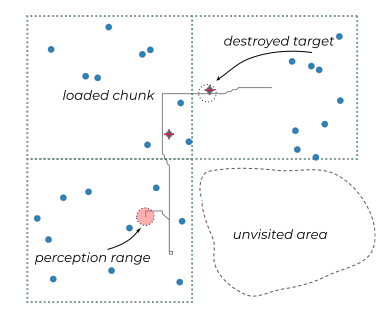
\includegraphics[width=0.55\textwidth]{images/chunks.png}
\caption{Schematic of the infinite-plane chunked world.  Square chunks (solid outlines) are loaded on demand as the forager moves; blue dots represent Poisson-distributed targets.  The perception range (dashed circle around the forager) defines the detection radius~$r_v$.  A destroyed target (crossed out) has been detected and removed in a previous flight.  The dashed region in the lower right indicates an unvisited area whose chunks have not yet been generated.}
\label{fig:chunks}
\end{figure}

\paragraph{Random number generation.}
All random variates (Poisson counts, uniform positions, flight
directions and lengths) are generated using the Mersenne Twister
(\texttt{mt19937}) seeded per-run from a master seed.
The chunk-level Poisson counts use a seed derived deterministically
from the chunk coordinates and the world seed, ensuring that
the target field is independent of the traversal order.

\subsection{Flight simulation}

For each $\mu$ value in the sweep $[\mu_{\min}, \mu_{\max}]$
with step~$\Delta\mu$:

\begin{enumerate}
  \item For each run $r = 1, \ldots, R$:
    \begin{enumerate}
      \item Initialize the forager at the origin.
            Regenerate the world (fresh PPP for each run).
      \item For each flight $n = 1, \ldots, N_{\mathrm{flights}}$:
        \begin{enumerate}
          \item Sample flight length $l \sim p(l;\mu)$ via
                \eqref{eq:inverse_cdf} and direction
                $\theta \sim \mathrm{Uniform}(0, 2\pi)$.
          \item Decompose the flight into segments of length
                $\Delta x$ (scan resolution).
          \item For each segment, load the relevant chunk and
                check all targets within detection radius~$r_v$
                of the segment centerline.
          \item Apply the post-detection strategy (no interrupt,
                teleport, or Viswanathan restart).
        \end{enumerate}
      \item Record $N_{\mathrm{unique}}^{(r)}$,
            $N_{\mathrm{visits}}^{(r)}$,
            $D_{\mathrm{total}}^{(r)}$,
            $D_{\mathrm{first}}^{(r)}$.
    \end{enumerate}
  \item Compute pooled metrics
        $\eta(\mu)$, $\lambda\eta(\mu)$, $\mathrm{MFPT}(\mu)$.
  \item Write results to CSV.
\end{enumerate}

\paragraph{Computation cost.}
A single $\mu$-sweep (21~values, $R = 120$ runs,
50\,000~flights each) completes in approximately
10--15~minutes on a single core (Intel Core~i7, 3.6\,GHz).
The full phase-diagram study (8~sparsity levels $\times$
4~strategies) required ${\sim}30$ CPU-hours in total.

\subsection{Default parameters}

\begin{table}[htb]
\centering
\begin{tabular}{llr}
\toprule
Parameter & Symbol & Default \\
\midrule
Vision radius         & $r_v$           & $0.5$ \\
Min flight length     & $l_{\min}$      & $r_v = 0.5$ \\
Max flight length     & $l_{\max}$      & $\lambda$ \\
Scan segment length   & $\Delta x$      & $50$ (in units of $r_v$: $100\,r_v$) \\
Chunk side            & $\Delta_{\mathrm{chunk}}$ & $2000$ \\
Teleport distance     & $l_c$           & $5\,r_v = 2.5$ \\
$\mu$ sweep           & $\mu_{\min}$--$\mu_{\max}$ & $1.0$--$3.0$ \\
$\mu$ step            & $\Delta\mu$     & $0.1$ \\
\bottomrule
\end{tabular}
\caption{Default simulation parameters.  The choice $r_v = 0.5$
         gives $\lambda = 1/\rho$, simplifying bookkeeping; all
         results are reported in dimensionless form
         ($\lambda/r_v$, $\lambda\eta$), so the particular value
         of~$r_v$ does not affect conclusions.}
\label{tab:defaults}
\end{table}

The density-dependent parameters (flights per run, number of runs)
vary with $\lambda/r_v$; see Table~\ref{tab:phase_params}
in Chapter~\ref{ch:experiments} for exact values.  As a rule,
$N_{\mathrm{flights}}$ ranges from 20\,000 (dense) to 150\,000
(sparse), and $R$ ranges from 100 to 120 for destructive and
300 to 360 for non-destructive strategies.

\paragraph{Scan resolution.}
The scan segment length $\Delta x = 50$ is much larger than
$r_v = 0.5$, but this does not cause missed detections: the
detection model checks whether any target center lies within
distance~$r_v$ of the straight-line segment, using the full
corridor geometry (rectangle of width~$2r_v$ plus endcaps).
Thus $\Delta x$ controls the frequency of chunk lookups, not
the detection fidelity.  To verify this, a comparison run was
performed at $\lambda/r_v = 100$ (destructive Viswanathan,
$\mu = 2.0$, $R = 50$) with $\Delta x = r_v = 0.5$: the
resulting $\lambda\eta = 0.469$ vs.\ $0.470$ with
$\Delta x = 50$, a relative difference of~$0.2\%$.

\paragraph{Flight budget.}
The search budget is specified as a fixed number of
flights~$N_{\mathrm{flights}}$ rather than a fixed total
distance.  Because the mean flight length $\langle l \rangle$
varies with~$\mu$, this means different $\mu$ values yield
different total distances.  We use the pooled
estimator~\eqref{eq:eta}, which normalizes by total distance
and is therefore invariant to this choice.  A fixed-distance
budget (terminating each run after a given distance) would
yield the same pooled~$\eta$ up to end-of-run boundary effects,
which are negligible for large $N_{\mathrm{flights}}$.

%-------------------------------------------------------------
\section{Truncation parameters}
\label{sec:truncation}

The standard choice $l_{\min} = r_v$, $l_{\max} = \lambda$
sets the scale of the shortest flights to the detection scale
and the longest flights to the mean free path.

To study the effect of truncation, we vary:
\begin{itemize}
  \item $l_{\max}/\lambda \in \{0.1,\,0.2,\,0.5,\,1,\,2,\,5,\,10\}$
        with fixed $l_{\min} = r_v$;
  \item $l_{\min}/r_v \in \{0.1,\,0.25,\,0.5,\,1,\,2,\,5\}$
        with fixed $l_{\max} = \lambda$.
\end{itemize}

%-------------------------------------------------------------
\section{Statistical methodology}
\label{sec:stat_method}

\subsection{Choice of runs}

The number of independent runs~$R$ for each $\mu$ value
is chosen to ensure convergence of the pooled estimator.
Convergence studies (Section~\ref{sec:convergence}) show that
$R \geq 50$ suffices for the destructive strategy, while
the non-destructive strategy requires $R \geq 200$ due to
the heavy-tailed distribution of per-run efficiency caused by
trapping.

\subsection{Optimal exponent extraction}

For each set of parameters, the optimal L\'evy exponent
$\mu^*$ is defined as the $\mu$ value that maximizes the
pooled unique-capture rate:
\begin{equation}
  \mu^* = \arg\max_{\mu} \lambda\eta(\mu).
  \label{eq:mu_star}
\end{equation}
The resolution of $\mu^*$ is limited by the $\mu$-grid step
$\Delta\mu = 0.1$.

\subsection{Uncertainty assessment}

Because the pooled estimator~\eqref{eq:eta} aggregates distance
and detections across all runs, individual error bars on
$\lambda\eta$ are not directly available from the pooled ratio.
Instead, uncertainty is assessed through convergence studies
(Section~\ref{sec:convergence}): $\lambda\eta(\mu)$ is computed
for increasing numbers of flights and runs, and the
variation of $\mu^*$ and $\lambda\eta_{\max}$ across these
subsamples quantifies the statistical stability of the results.
For the destructive strategy, $\lambda\eta_{\max}$ converges
within $0.5\%$ at $R \geq 50$.  For the non-destructive
strategy, $\mu^*$ remains noisy ($\pm 0.3$--$0.5$) even at
$R = 400$, although $\lambda\eta_{\max}$ converges within $1\%$
at $R \geq 200$.  These convergence envelopes effectively serve
as uncertainty bounds on the reported values.

%-------------------------------------------------------------
\section{Analytical benchmark}
\label{sec:analytical_theory}

As an analytical benchmark we use the mean-field model of
Viswanathan et~al.~\cite{viswanathan1999optimizing}.  The
unique-capture rate is approximated as
\begin{equation}
  \eta \;\approx\; \frac{1}{\langle l \rangle_{\mathrm{MF}}
  \cdot N(\mu)},
  \label{eq:eta_analytical}
\end{equation}
where $\langle l \rangle_{\mathrm{MF}}$ is a mean-field
mean flight distance and $N(\mu)$ is the mean number of
flights between successive target encounters.

The mean-field flight distance
(Viswanathan~et~al.\ eq.~2) treats flights longer than
$\lambda$ as contributing $\lambda$ (mean-field truncation):
\begin{equation}
  \langle l \rangle_{\mathrm{MF}} = r_v \left[
    \frac{(\mu-1)(R^{2-\mu}-1)}{2-\mu} + R^{2-\mu}
  \right], \qquad R = \lambda/r_v,\; \mu \neq 1,2.
  \label{eq:mean_l_mf}
\end{equation}
Limiting cases: $\langle l \rangle_{\mathrm{MF}} = \lambda$
for $\mu = 1$ and
$\langle l \rangle_{\mathrm{MF}} =
r_v(\ln R + 1)$ for $\mu = 2$.

The encounter scaling
(Viswanathan~et~al.\ eq.~5) gives
\begin{equation}
  N(\mu) = \left(\frac{\lambda}{r_v}\right)^{(\mu-1)/2},
  \label{eq:N_visw}
\end{equation}
so that the dimensionless efficiency is
$\lambda\eta \approx C \cdot
\lambda / (\langle l \rangle_{\mathrm{MF}} \cdot N)$,
where the proportionality constant~$C$ is fitted by
least squares to the simulation data.

\paragraph{Qualitative behavior.}
For $\mu < 2$,
$\langle l \rangle_{\mathrm{MF}}$ grows as
$R^{2-\mu}$ while $N$ is moderate, so $\eta$ decreases
toward the ballistic limit ($\mu \to 1$).
For $\mu > 2$,
$\langle l \rangle_{\mathrm{MF}}$ saturates near~$r_v$,
but $N$ grows as $R^{(\mu-1)/2}$, penalizing short-flight
strategies for trajectory self-intersection (revisiting
cleared areas).  The product
$\langle l \rangle_{\mathrm{MF}} \cdot N$ is therefore
minimized near $\mu \approx 2$, predicting the efficiency
peak at the L\'evy--Brownian transition.

\paragraph{Limitations.}
The encounter exponent~\eqref{eq:N_visw} was originally
derived for the non-destructive case; it is applied here
as an approximation to the destructive Viswanathan strategy
under the assumption that trajectory self-intersection
(the dominant correction in 2D) follows similar scaling.
The model overestimates efficiency for $\mu > 2.5$
(Section~\ref{sec:analytical_comparison}), where the
penalty for oversampling by very short flights exceeds the
$N(\mu)$ correction.